\documentclass[a4paper]{beamer}

\definecolor{fudepan}{HTML}{006c63}
\definecolor{verde}{RGB}{0, 127, 63}
\definecolor{gris}{RGB}{86, 86, 86}
\definecolor{listinggray}{gray}{0.9}
\definecolor{lbcolor}{rgb}{0.95,0.95,0.95}

\mode<presentation>{
  \usetheme{Warsaw}		
  \usecolortheme[named=verde]{structure}
  \setbeamercovered{transparent}	
}

\usepackage[spanish]{babel} 
\usepackage[utf8]{inputenc} 
\usepackage{graphicx}
\usepackage{amsmath}
\usepackage{verbatim}
\usepackage{listings}
\usepackage[dvips,final]{epsfig}
\usepackage{color}
\usepackage{amssymb}
\usepackage{listings}
\usepackage{hyperref} 

\definecolor{gray97}{gray}{.97}
\definecolor{gray75}{gray}{.75}
\definecolor{gray45}{gray}{.45}

\lstset{ frame=TRBL,
     frameround=tttt,
     framerule=0pt,
     aboveskip=0.5cm,
     framextopmargin=3pt,
     framexbottommargin=3pt,
     framexleftmargin=0.4cm,
     framesep=0pt,
     rulesep=.4pt,
     backgroundcolor=\color{gray97},
     rulesepcolor=\color{black},     
     commentstyle=\text
     stringstyle=\ttfamily,
     showstringspaces = false,
     basicstyle=\tiny,%\ttfamily,
     commentstyle=\color{gray45},
     keywordstyle=\bfseries,
   }

\definecolor{listinggray}{gray}{0.9}
\definecolor{lbcolor}{rgb}{0.95,0.95,0.95}
\lstset{
    backgroundcolor=\color{lbcolor},
    tabsize=4,
    rulecolor=,
    language=matlab,
        basicstyle=\scriptsize,
        upquote=true,
        aboveskip={1.5\baselineskip},
        columns=fixed,
        showstringspaces=false,
        extendedchars=true,
        breaklines=true,
        prebreak = \raisebox{0ex}[0ex][0ex]{\ensuremath{\hookleftarrow}},
        frame=single,
        showtabs=false,
        showspaces=false,
        showstringspaces=false,
        identifierstyle=\ttfamily,
        keywordstyle=\color[rgb]{0.1,0.1,0.6}\bfseries,
        commentstyle=\color[rgb]{0.133,0.545,0.133},
        stringstyle=\color[rgb]{0.627,0.126,0.941},
}

%---------------------------- Presentacion--------------------------------------- 
\title[Reunión Científica Anual de la Sociedad Argentina de Virología]{Estudio de la relación entre \emph{divergencia}  en el uso de codones del virus respecto al  huésped y \emph{reconocimiento} por los $\mu$RNA}

\author[Riberi, Fazzi, Tardivo, Gutson, Rabinovich]{Franco Riberi\inst{1,3} \and Fazzi Lucía\inst{2} \and Tardivo Laura\inst{3} \\ \and Gutson Daniel\inst{1} \and Rabinovich Daniel\inst{1,2}}

\institute{\tiny{${^1}$Fundación para el Desarrollo de la Programación en Ácidos Nucleicos-FuDePAN, Córdoba, Argentina. \and ${^2}$Instituto de Investigaciones Biomédicas en Retrovirus y SIDA (UBA-CONICET).
(INBIRS), Buenos Aires, Argentina.  \and ${^3}$ Departamento de Computaci\'on, FCEFQyN, Universidad Nacional de Río Cuarto, Río Cuarto, Córdoba, Argentina}
\\
\begin{minipage}{0.25\textwidth}
\begin{center} 
\vskip .2 cm

\includegraphics[width=25pt,height=35pt]{image/unrc.jpg}
\end{center} 
\end{minipage}
\begin{minipage}{0.2\textwidth}
\begin{center} 
\vskip .2 cm
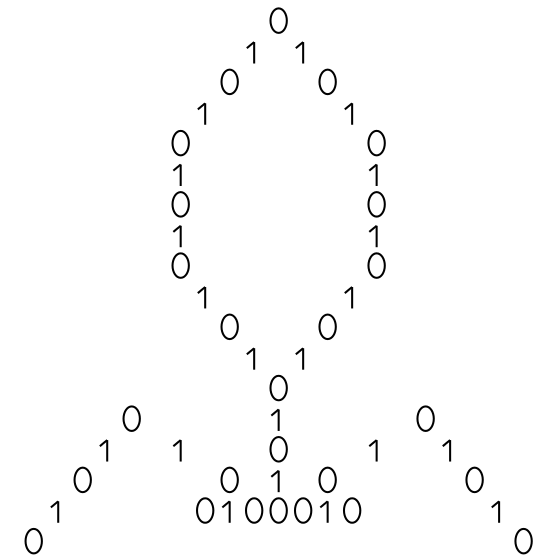
\includegraphics[width=35pt,height=30pt]{image/fudepan.png} \\
\begin{tiny}\textsc{FuDePAN}\end{tiny}
\end{center}
\end{minipage}
\begin{minipage}{0.2\textwidth}
\begin{center} 
\vskip .2 cm

\includegraphics[width=35pt,height=30pt]{image/dani.jpg}
\end{center}
\end{minipage}
}

\date{06 de Diciembre de 2012}
%--------------------------indice o temario---------------------------- 
\begin{document}
   \frame{\titlepage}

\section{Introducción}
\begin{frame}
    \frametitle{Introducción}
        \begin{block}{Planteo problema}           
                 Divergencia en el ``uso'' de codones entre el optimo para el hospedero y el virus.
                 %Intentar comprender el porque de esta divergencia               
                %optimo para el hospedero: el humano en este casos

        \end{block}
        \begin{block}{Utilidad}                           
                Comprender la evolución de los virus y diseño de secuencias (vacunales, interferentes) más   eficientes.
        \end{block}

        \begin{block}{Algunas teorías propuestas}
            \begin{itemize}
                \item Regulación fina de la síntesis proteica.
	            \item Asociación a la proporción \emph{G-C} en el DNA.
	            \item Estabilidad para soportar mutaciones.
	            \item Presión mutacional.
            \end{itemize}
        \end{block}
\end{frame}

\begin{frame}
    \frametitle{Objetivos}
        \begin{block}{Objetivo parte 1}
            Estudiar la relación entre \emph{DIVERGENCIA} y \emph{RECONOCIMIENTO por $\mu$RNAs}.    
        \end{block}
        \begin{block}{Objetivo parte 2}            
            Estudiar la relación entre \emph{DIVERGENCIA} y \emph{estructura secundaria}.
        \end{block}
\end{frame}

\section{Primer Objetivo}
\begin{frame}
    \frametitle{Primer Objetivo}
    Ejemplificando con \emph{influenza (segmento 5)}, \emph{polio1}, \emph{sarampión}, \emph{adenovirus} y 50 $\mu$RNAs.
	\begin{itemize}
        \item Se optimizó el uso de codones (\emph{GeneDesign}) para h.sapiens.
        \item Se comparó (método ad-hoc, RNAup, IntaRNA, herramientas de mirBase). 
    \end{itemize}   
    \vskip 1cm
    \hspace*{2cm} [sec. orig mensajero] como blanco de [$\mu$RNA] \\
    \hspace*{5cm} versus \\
    \hspace*{2cm} $[$sec. opt. mensajero$]$ como blanco de [$\mu$RNA] 
\end{frame}

\begin{frame}
    \frametitle{Resultados (Cont.)}
\begin{center}
\resizebox{9cm}{!}{
	\begin{tabular}{| c | c | c | c |}
   	\hline
      {\bf Método} & {\bf } & {\bf Enretovirus C} & {\bf Influenza} \\
      \hline
      \hline
       %clara tendecsia 
       Ad-hoc &  & &  & \hline 	
       & \% sitios mejor reconocidos en el opt. & 42.8\% & 53.92\% &  \hline 		 
       & \% sitios en que dio opt = orig. & 32.15\% & 25.90\%  & \hline
       & \% sitios mejor reconocidos en el orig. & 25.04\% & 20.18\% & \hline
       \hline
       IntaRNA &  & &  & \hline 	
       & \% $\mu$RNA reconocen opt. & ? & 70\% &  \hline 		 
       & \% $\mu$RNA reconocen orig. & ?  & 30\% & \hline
       \hline
       RNAup &  & &  & \hline 	
       & \% $\mu$RNA reconocen opt. & ?  & 70\% &  \hline 		 
       & \% $\mu$RNA reconocen orig. & ? & 30\% &        
      \hline
	\end{tabular}
}
    \begin{alertblock}{Resultados}
    \small{
    Cambios masivos en el patrón de reconocimiento de los $\mu$RNA en orig/opt.:
        \begin{itemize}
		    \item RNAup \& IntaRNA: 70\% uRNAs reconocen mejor opt. que orig.
%		%("si virus se humanizara, sería más susceptible a la acción de los uRNA").
		    \item mirBASE (E con corte=11) reconoce (58 opt, 30 orig). %sarampion, adenovirus  
    		\item Tendencia visible también en método ad-hoc.
        \end{itemize}                
    }
    \end{alertblock}    
\end{center}
\end{frame}

\section{Segundo Objetivo}
\begin{frame}
    \frametitle{Segundo Objetivo}
    Comparación de: Estructura secundaria del RNA$_m$ orig. y del RNA$_m$ optimizado.
    %objetivos relacion entre divergenci y estructura    
    \begin{block}{Resultados Influenza}
        \begin{center}
	        \begin{tabular}{| c | c | c |}
           	\hline
                %segmento doble cadena
              {\bf $_d$$_s$RNA size} & {\bf Original} & {\bf Optimizado} \\
              \hline
              \hline               
               11 & 0 & 1 & \hline 	
               10 & 1 & 1 &  \hline 		 
               9  & 3 & 3 & \hline
               8  & 2 & 5 & \hline
%               7  & 5 & 7 & \hline
	        \end{tabular}
%            tendencia de segmentos de doble hélice con tamaño size en el opt.              
\end{center}
    \end{block}
\end{frame}

\section{Conclusiones}
\begin{frame}
    \frametitle{Conclusiones}
        \begin{itemize}
            \item Se produce un profundo cambio en el patron de $\mu$RNA capaces de ser efectivos.
            \item Se puede producir un aumento del número de $\mu$RNA. 

            \item Existe una tendencia en los virus estudiados de que al optimizar el virus se generen nuevos 
            blancos para $\mu$RNA.

            \item Las secuencias optimizadas poseen mayor cantidad de segmentos de mayor longitud apareados en la estructura secundaria que podrían favorecer la producción de \emph{interferón}.
       \end{itemize}
        \begin{alertblock}{Conclusión general}
            La DIVERGENCIA en el uso de codones respecto al óptimo para la traducción puede estar relacionada tanto con el \emph{patrón de blancos para los $\mu$RNA} como con la \emph{estructura secundaria del RNA}.             
        \end{alertblock}
\end{frame}

\begin{frame}
\frametitle{Preguntas}
	\begin{center}
		
\includegraphics[height=5cm]{image/preguntas.jpg}
	\end{center}
\end{frame}			

\begin{frame}
\frametitle{}
	\begin{center}
		Muchas Gracias por su atención!!!
	\end{center}
\end{frame}			

\end{document}
